\documentclass[10pt]{beamer}

\usepackage[utf8]{inputenc}
%\usepackage[russian,polish]{babel}
\usepackage[T2A]{fontenc}
\usepackage{graphicx}
\usepackage{animate}
\usepackage{hyperref}
\usepackage[main=polish,russian]{babel}
\usepackage{csquotes}

\hypersetup{
    colorlinks=true,
    linkcolor=[RGB]{214, 2, 73},
    filecolor=magenta,
    urlcolor=[RGB]{173, 2, 230},
    pdftitle={prez},
    pdfpagemode=FullScreen,
}

\usetheme{Warsaw}
\usecolortheme{albatross}

\title{Plazma}
\subtitle{Elektrostatyczne utrzymywanie plazmy i Inercyjne wywoływanie reakcji}
\author{Maciej Jerzyk, Mikołaj Krenc}
\date{21.01.2025r.}

\begin{document}

    \begin{frame}
        \titlepage{}
    \end{frame}

    \begin{frame}{Spis Treści}
        \tableofcontents
    \end{frame}

    \section{Wprowadzenie}

        \begin{frame}{Co to jest plazma?}
            \begin{itemize}
                \item \textbf{Plazma} - jedna z czterech podstawowych stanów materii charakteryzująca się dużą koncentracją jonów.
                \item Jednym ze sposobów otrzymywania plazmy jest podgrzanie materii do wysokiej temperatury, mowa tu o temperaturach sięgających 10000\ K. Energia elektronu w plazmie o wysokiej temperaturze może wynosić aż 100\ eV!
                \item Inne techniki otrzymywania plazmy wykorzystują pole magnetyczne.
            \end{itemize}

            \raggedright{}
            \includegraphics[width=0.4\textwidth]{plasma.jpg}

        \end{frame}

        \begin{frame}{Plazma powstająca w naturze nierzadko osiąga takie, i dużo wyższe parametry i trwale się utrzymuje.}
            \begin{minipage}{0.49\textwidth}
                \centering
                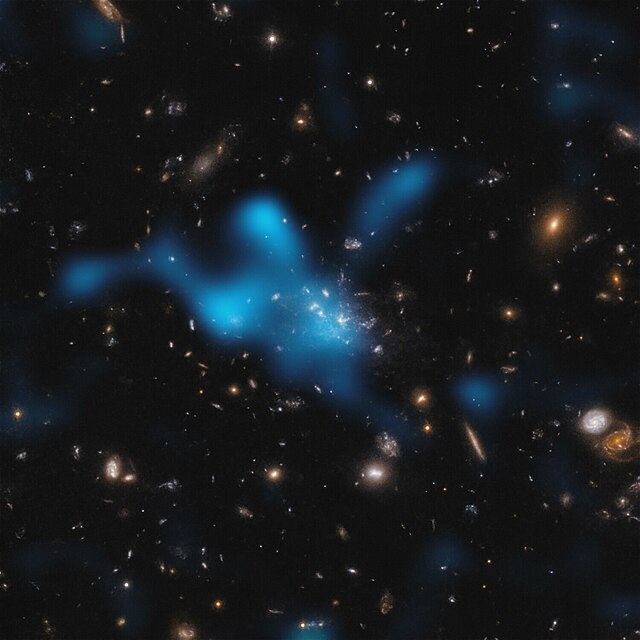
\includegraphics[width=0.8\linewidth]{intracluster.jpg}
            \end{minipage}
            \hfill
            \begin{minipage}{0.49\textwidth}
                \centering
                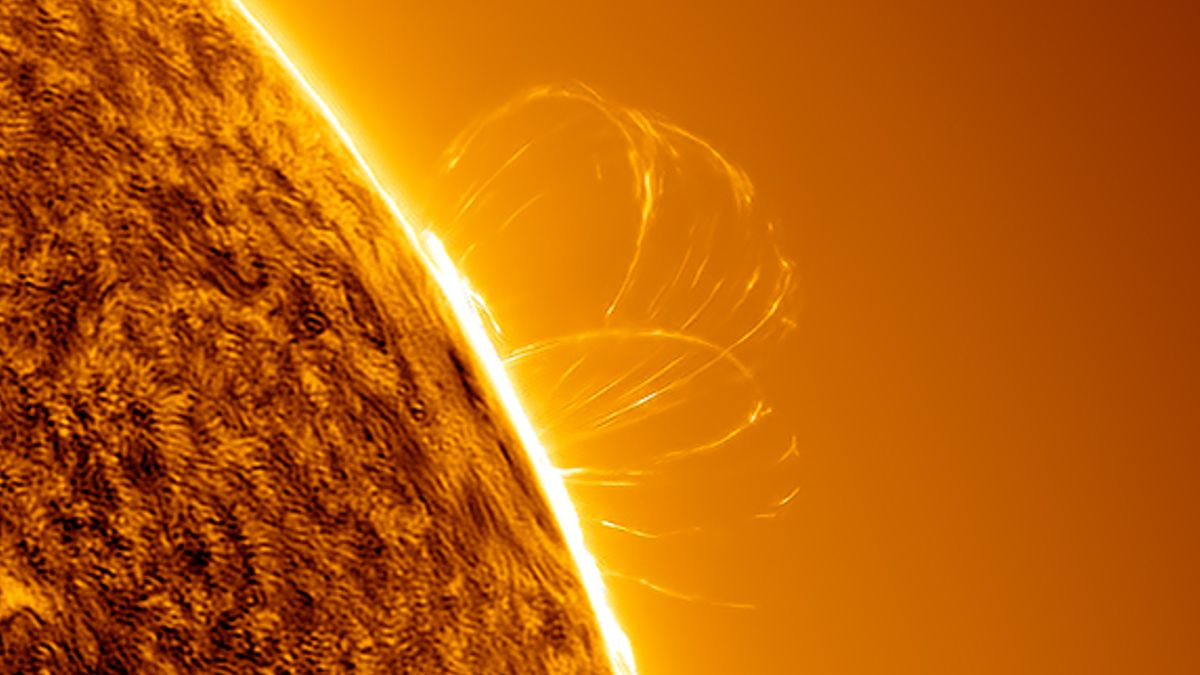
\includegraphics[width=0.8\linewidth]{star.jpg}
            \end{minipage}
        \end{frame}

        \begin{frame}{Ale my musimy się jeszcze wiele nauczyć\dots}
            \begin{minipage}{0.49\textwidth}
                \centering
                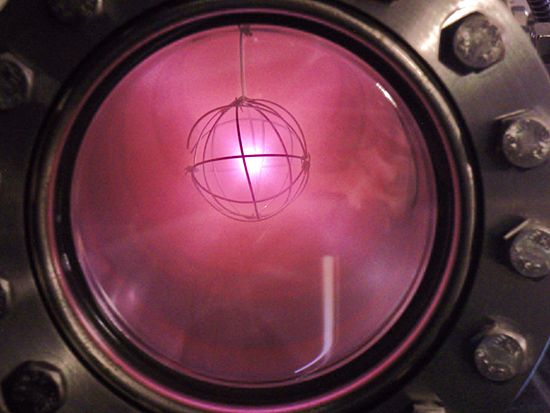
\includegraphics[width=0.8\linewidth]{deuterium.jpg}
            \end{minipage}
            \hfill
            \begin{minipage}{0.49\textwidth}
                \centering
                
\includegraphics[width=0.8\linewidth]{patrick.jpeg}
            \end{minipage}
        \end{frame}

    \begin{frame}{Gdzie znajdziemy plazmę w technice?}
        Plazmę można wytwarzać np.\ w maszynach typu \textbf{Tokamak} (ros. \foreignlanguage{russian}{тороидальная камера с магнитными катушками},\ trb.\ \textbf{to}roidalnaja \textbf{ka}miera s \textbf{ma}gnitnymi \textbf{k}atuszkami -\ „toroidalna komora z cewką magnetyczną”), powstaje ona też w fuzorach. Plazmę znajdziemy w technice jeszcze w wielu innych miejscach.
        \begin{minipage}{0.49\textwidth}
            \centering
            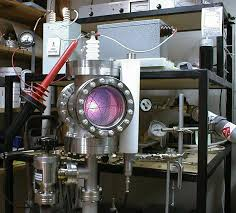
\includegraphics[width=0.8\linewidth]{fusor.jpeg}
        \end{minipage}
        \hfill
        \begin{minipage}{0.49\textwidth}
            \centering
            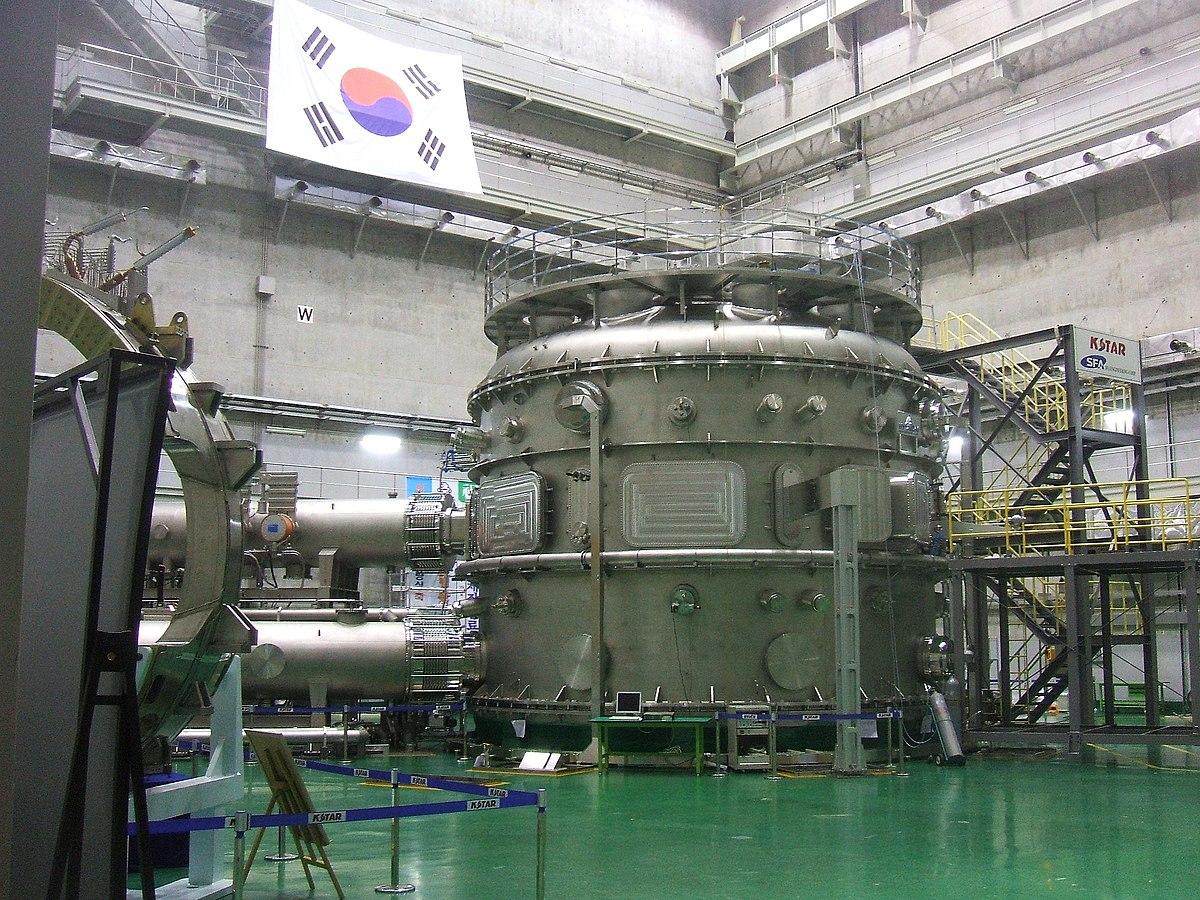
\includegraphics[width=0.8\linewidth]{tokamak.jpg}
        \end{minipage}
        Ale właściwie po co nam ta plazma?
    \end{frame}

    \begin{frame}{A komu to potrzebne?}
        Przykłady z poprzedniego slajdu ilustrowały dwa przypadki, w których plazma pojawia się w technice:
        \begin{itemize}
            \item kiedy zależy nam na utrzymaniu plazmy,
            \item kiedy powstawanie plazmy jest efektem ubocznym lub posiłkowym.
        \end{itemize}
        Tak naprawdę, w większości przypadków, jak stanie się to jasne w toku tej prezentacji, te dwa warianty zleją się w jeden, gdy okaże się, że prawie zawsze, a szczególnie w Fizyce jądrowej, powstanie plazmy jest co najwyżej celem pośrednim. Powiemy jeszcze przedtem o tych kilku wyjątkowych przykładach.
    \end{frame}

    \begin{frame}{Ludzka ciekawość; bajery\dots}
        \begin{minipage}{0.49\textwidth}
            \centering
            
\includegraphics[width=0.8\linewidth]{patrick.png}
        \end{minipage}
        \hfill
        \begin{minipage}{0.49\textwidth}
            \centering
            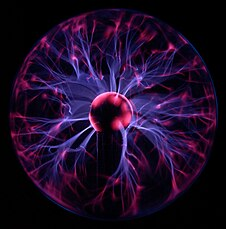
\includegraphics[width=0.8\linewidth]{lamp.jpg}
        \end{minipage}
    \end{frame}

    \section{Synteza jądrowa w pułapce inercyjnej}

        \begin{frame}{Kapsułka paliwowa}
            Kluczowym elementem pułapki inercyjnej jest przygotowanie kapsułki paliwowej.
            Przyglądając się koncentrycznej strukturze przekroju kapsułki można zobaczyć:
            \begin{itemize}
                \item \textbf{Warstwę ablacyjną},
                \item \textbf{Lód deuterowo-trytowy},
                \item \textbf{Gazowe wypełnienie deuterowo-trytowe}.
            \end{itemize}
            \begin{minipage}{0.49\textwidth}
                \centering
                \includegraphics[width=0.8\linewidth]{eye.jpg}
            \end{minipage}
            \hfill
            \begin{minipage}{0.49\textwidth}
                \centering
                \includegraphics[width=0.8\linewidth]{caps.png}
            \end{minipage}
        \end{frame}

    \section{Metoda elektrostatycznego inercyjnego utrzymywania plazmy}

    \begin{frame}{Na czym polega metoda inercyjna?}
        Ogólna metoda inercyjna pozwala wytwarzać plazmę przez chwilowe ściśnięcie 
        % \begin{itemize}
        %     \item 
        % \end{itemize}
    \end{frame}

    \begin{frame}{Historia metody inercyjnej}

    \end{frame}


\end{document}
